\fcolorbox{orange}{white}{
\begin{minipage}[t]{242mm}
\vspace{5mm}\section*{\fontsize{48}{20}\selectfont Parsing} \vspace{-3mm}
\subsection*{\fontsize{40}{20}\selectfont Parsing tree}
\linespread{1.9}\fontsize{32}{20}\sffamily\selectfont
\color[cmyk]{0,0,0,1}
\begin{center}\begin{tabular}{lcl}
\vspace{70mm}Interpreted structure & & Statements \\
 & & Input: \\
 & & \ A(B(\#1C),\$\#1(D)) \\
 & & Output: \\
 & & \ A(B(\#1C),\$\#1@\#1C(D)) \\
\raisebox{\baselineskip}[0pt][0pt]{
\epsfig{file=t1ig.eps,height=130mm}} & &  \\
\end{tabular}\end{center}
\color[cmyk]{1,1,0,0.8}

\subsection*{\fontsize{40}{20}\selectfont Parsing graph}
\vspace{5mm}
\linespread{1.9}\fontsize{32}{20}\sffamily\selectfont
\color[cmyk]{0,0,0,1}
\begin{center}\begin{tabular}{lcl}
\multicolumn{3}{c}{\textbf{Implicit graph}}\\
\vspace{28mm}Interpreted structure & & Statements \\
 & & Input:\\
 & & \ A(B(\#1C),\$\#1(D)) \\
 & & Adjacency matrix:\\
 & & \ [:A:0],1,2,3,,\\
 & & \ ,[:B:1],2,,,\\
 & & \ ,,[:\#1C:2],,,\\
 & & \ ,,,[:\$\#1:3$\rightarrow$2],4,\\
 & & \ ,,,,[:D:4],\\
\raisebox{\baselineskip}[0pt][0pt]{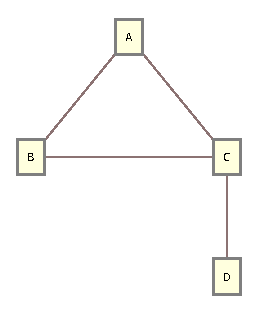
\epsfig{file=t2ig.eps,height=140mm}} & &  \\
\end{tabular}\end{center}

\vspace{5mm}
\begin{center}\begin{tabular}{lcp{100mm}}
\multicolumn{3}{c}{\textbf{Explicit graph}}\\
\vspace{7mm}Interpreted structure & & Statements \\
 & & \hspace{-3mm}Input:\\
 & & \linespread{1.2}\fontsize{20}{20}\sffamily\selectfont \$G\$(\$V\$(\#0,\#1,\#2), \$E\$(\$\#0(\$\#1,\$\#2), \$\#1(\$\#0,\$\#2), \$\#2(\$\#0,\$\#1)))\\
 & & \hspace{-3mm}Adjacency matrix:\\
 & & \linespread{1.2}\fontsize{20}{20}\sffamily\selectfont 
,,,3,4,,[:\$\#0:6$\rightarrow$2],7,8,,,,,,,
,,,,,,,[:\$\#1:7$\rightarrow$3],,,,,,,,
,,,,,,,,[:\$\#2:8$\rightarrow$4],,,,,,,
,,2,,4,,,,,[:\$\#1:9$\rightarrow$3],10,11,,,,
,,,,,,,,,,[:\$\#0:10$\rightarrow$2],,,,,
,,,,,,,,,,,[:\$\#2:11$\rightarrow$4],,,,
,,2,3,,,,,,,,,[:\$\#2:12$\rightarrow$4],13,14,
,,,,,,,,,,,,,[:\$\#0:13$\rightarrow$2],,
,,,,,,,,,,,,,,[:\$\#1:14$\rightarrow$3], \vspace{-10mm}\\
\raisebox{\baselineskip}[0pt][0pt]{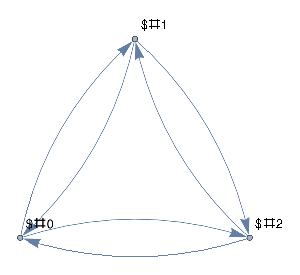
\epsfig{file=gr1.eps,height=120mm}} & &  \\
\end{tabular}\end{center}


\subsection*{\fontsize{40}{20}\selectfont Binding and reforming data} \vspace{-3mm}
\linespread{1.9}\fontsize{32}{20}\sffamily\selectfont
\color[cmyk]{0,0,0,1}
\begin{center}\begin{tabular}{lcp{100mm}}
\vspace{4mm}Interpreted structure & & Statements \\
 & & \hspace{-3mm}Input:\\
 & & \linespread{1.2}\fontsize{20}{20}\sffamily\selectfont (\#1\$1[2],\#2\$2[2],\$3[3](\#4\$4[2])); \$PI\$(\$\#1,Quantity(\$\#4,\$\#2)) \\
 & & \hspace{-3mm}Data:\\
 & & \linespread{1.2}\fontsize{20}{20}\sffamily\selectfont 
Length,Weight,
mm,kg,
1,2,
322,4,
5,68\\
 & & \hspace{-3mm}Output:\\
 & & \linespread{1.2}\fontsize{20}{20}\sffamily\selectfont (((Length,Quantity(1,mm)), (Weight,Quantity(2,kg))), ((Length,Quantity(322,mm)), (Weight,Quantity(4,kg))), ((Length,Quantity(5,mm)), (Weight,Quantity(68,kg)))) \vspace{-12mm}\\
\raisebox{\baselineskip}[0pt][0pt]{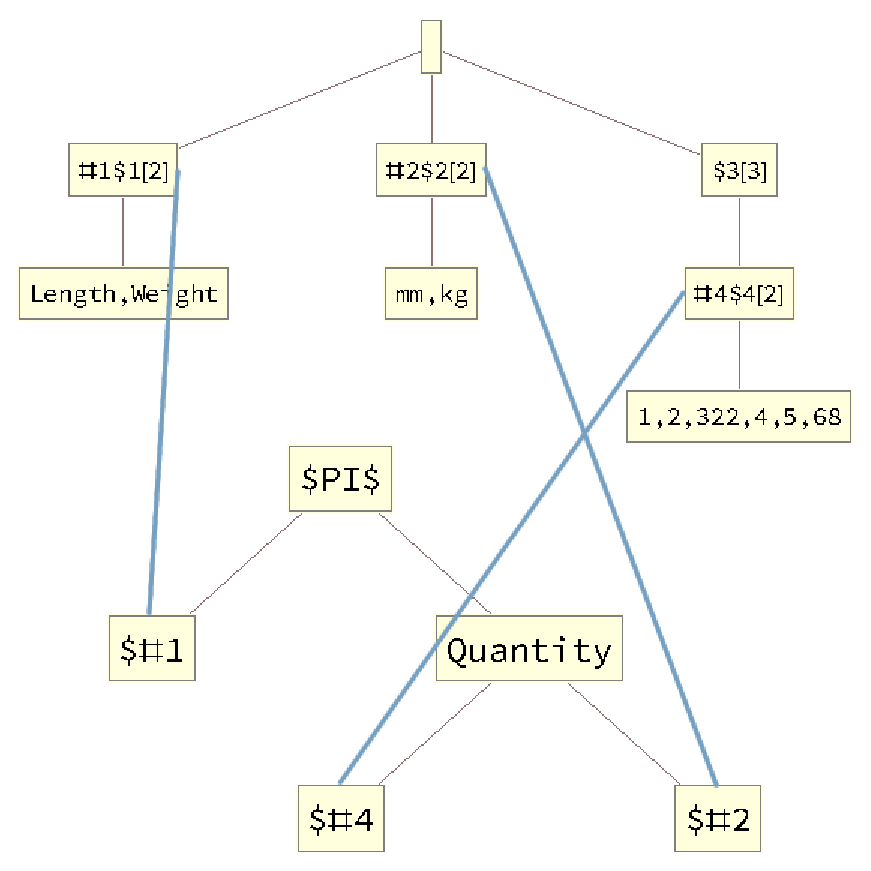
\epsfig{file=gdb2-2.eps,height=130mm}} & &  \\
%\raisebox{\baselineskip}[0pt][0pt]{\epsfig{file=gdb2-1.eps,height=110mm}} & &  \\
%\raisebox{\baselineskip}[0pt][0pt]{\epsfig{file=gdb2.eps,height=110mm}} & &  \\
%\raisebox{\baselineskip}[0pt][0pt]{\epsfig{file=fig-graph-bind.eps,height=110mm}} & &  \\
\end{tabular}\end{center}
\vspace{0.01mm}
\end{minipage} }

